% Options for packages loaded elsewhere
\PassOptionsToPackage{unicode}{hyperref}
\PassOptionsToPackage{hyphens}{url}
\PassOptionsToPackage{dvipsnames,svgnames,x11names}{xcolor}
%
\documentclass[
  letterpaper,
  DIV=11,
  numbers=noendperiod]{scrartcl}

\usepackage{amsmath,amssymb}
\usepackage{lmodern}
\usepackage{iftex}
\ifPDFTeX
  \usepackage[T1]{fontenc}
  \usepackage[utf8]{inputenc}
  \usepackage{textcomp} % provide euro and other symbols
\else % if luatex or xetex
  \usepackage{unicode-math}
  \defaultfontfeatures{Scale=MatchLowercase}
  \defaultfontfeatures[\rmfamily]{Ligatures=TeX,Scale=1}
\fi
% Use upquote if available, for straight quotes in verbatim environments
\IfFileExists{upquote.sty}{\usepackage{upquote}}{}
\IfFileExists{microtype.sty}{% use microtype if available
  \usepackage[]{microtype}
  \UseMicrotypeSet[protrusion]{basicmath} % disable protrusion for tt fonts
}{}
\makeatletter
\@ifundefined{KOMAClassName}{% if non-KOMA class
  \IfFileExists{parskip.sty}{%
    \usepackage{parskip}
  }{% else
    \setlength{\parindent}{0pt}
    \setlength{\parskip}{6pt plus 2pt minus 1pt}}
}{% if KOMA class
  \KOMAoptions{parskip=half}}
\makeatother
\usepackage{xcolor}
\setlength{\emergencystretch}{3em} % prevent overfull lines
\setcounter{secnumdepth}{-\maxdimen} % remove section numbering
% Make \paragraph and \subparagraph free-standing
\ifx\paragraph\undefined\else
  \let\oldparagraph\paragraph
  \renewcommand{\paragraph}[1]{\oldparagraph{#1}\mbox{}}
\fi
\ifx\subparagraph\undefined\else
  \let\oldsubparagraph\subparagraph
  \renewcommand{\subparagraph}[1]{\oldsubparagraph{#1}\mbox{}}
\fi

\usepackage{color}
\usepackage{fancyvrb}
\newcommand{\VerbBar}{|}
\newcommand{\VERB}{\Verb[commandchars=\\\{\}]}
\DefineVerbatimEnvironment{Highlighting}{Verbatim}{commandchars=\\\{\}}
% Add ',fontsize=\small' for more characters per line
\usepackage{framed}
\definecolor{shadecolor}{RGB}{241,243,245}
\newenvironment{Shaded}{\begin{snugshade}}{\end{snugshade}}
\newcommand{\AlertTok}[1]{\textcolor[rgb]{0.68,0.00,0.00}{#1}}
\newcommand{\AnnotationTok}[1]{\textcolor[rgb]{0.37,0.37,0.37}{#1}}
\newcommand{\AttributeTok}[1]{\textcolor[rgb]{0.40,0.45,0.13}{#1}}
\newcommand{\BaseNTok}[1]{\textcolor[rgb]{0.68,0.00,0.00}{#1}}
\newcommand{\BuiltInTok}[1]{\textcolor[rgb]{0.00,0.23,0.31}{#1}}
\newcommand{\CharTok}[1]{\textcolor[rgb]{0.13,0.47,0.30}{#1}}
\newcommand{\CommentTok}[1]{\textcolor[rgb]{0.37,0.37,0.37}{#1}}
\newcommand{\CommentVarTok}[1]{\textcolor[rgb]{0.37,0.37,0.37}{\textit{#1}}}
\newcommand{\ConstantTok}[1]{\textcolor[rgb]{0.56,0.35,0.01}{#1}}
\newcommand{\ControlFlowTok}[1]{\textcolor[rgb]{0.00,0.23,0.31}{#1}}
\newcommand{\DataTypeTok}[1]{\textcolor[rgb]{0.68,0.00,0.00}{#1}}
\newcommand{\DecValTok}[1]{\textcolor[rgb]{0.68,0.00,0.00}{#1}}
\newcommand{\DocumentationTok}[1]{\textcolor[rgb]{0.37,0.37,0.37}{\textit{#1}}}
\newcommand{\ErrorTok}[1]{\textcolor[rgb]{0.68,0.00,0.00}{#1}}
\newcommand{\ExtensionTok}[1]{\textcolor[rgb]{0.00,0.23,0.31}{#1}}
\newcommand{\FloatTok}[1]{\textcolor[rgb]{0.68,0.00,0.00}{#1}}
\newcommand{\FunctionTok}[1]{\textcolor[rgb]{0.28,0.35,0.67}{#1}}
\newcommand{\ImportTok}[1]{\textcolor[rgb]{0.00,0.46,0.62}{#1}}
\newcommand{\InformationTok}[1]{\textcolor[rgb]{0.37,0.37,0.37}{#1}}
\newcommand{\KeywordTok}[1]{\textcolor[rgb]{0.00,0.23,0.31}{#1}}
\newcommand{\NormalTok}[1]{\textcolor[rgb]{0.00,0.23,0.31}{#1}}
\newcommand{\OperatorTok}[1]{\textcolor[rgb]{0.37,0.37,0.37}{#1}}
\newcommand{\OtherTok}[1]{\textcolor[rgb]{0.00,0.23,0.31}{#1}}
\newcommand{\PreprocessorTok}[1]{\textcolor[rgb]{0.68,0.00,0.00}{#1}}
\newcommand{\RegionMarkerTok}[1]{\textcolor[rgb]{0.00,0.23,0.31}{#1}}
\newcommand{\SpecialCharTok}[1]{\textcolor[rgb]{0.37,0.37,0.37}{#1}}
\newcommand{\SpecialStringTok}[1]{\textcolor[rgb]{0.13,0.47,0.30}{#1}}
\newcommand{\StringTok}[1]{\textcolor[rgb]{0.13,0.47,0.30}{#1}}
\newcommand{\VariableTok}[1]{\textcolor[rgb]{0.07,0.07,0.07}{#1}}
\newcommand{\VerbatimStringTok}[1]{\textcolor[rgb]{0.13,0.47,0.30}{#1}}
\newcommand{\WarningTok}[1]{\textcolor[rgb]{0.37,0.37,0.37}{\textit{#1}}}

\providecommand{\tightlist}{%
  \setlength{\itemsep}{0pt}\setlength{\parskip}{0pt}}\usepackage{longtable,booktabs,array}
\usepackage{calc} % for calculating minipage widths
% Correct order of tables after \paragraph or \subparagraph
\usepackage{etoolbox}
\makeatletter
\patchcmd\longtable{\par}{\if@noskipsec\mbox{}\fi\par}{}{}
\makeatother
% Allow footnotes in longtable head/foot
\IfFileExists{footnotehyper.sty}{\usepackage{footnotehyper}}{\usepackage{footnote}}
\makesavenoteenv{longtable}
\usepackage{graphicx}
\makeatletter
\def\maxwidth{\ifdim\Gin@nat@width>\linewidth\linewidth\else\Gin@nat@width\fi}
\def\maxheight{\ifdim\Gin@nat@height>\textheight\textheight\else\Gin@nat@height\fi}
\makeatother
% Scale images if necessary, so that they will not overflow the page
% margins by default, and it is still possible to overwrite the defaults
% using explicit options in \includegraphics[width, height, ...]{}
\setkeys{Gin}{width=\maxwidth,height=\maxheight,keepaspectratio}
% Set default figure placement to htbp
\makeatletter
\def\fps@figure{htbp}
\makeatother

\usepackage{booktabs}
\usepackage{longtable}
\usepackage{array}
\usepackage{multirow}
\usepackage{wrapfig}
\usepackage{float}
\usepackage{colortbl}
\usepackage{pdflscape}
\usepackage{tabu}
\usepackage{threeparttable}
\usepackage{threeparttablex}
\usepackage[normalem]{ulem}
\usepackage{makecell}
\usepackage{xcolor}
\KOMAoption{captions}{tableheading}
\makeatletter
\makeatother
\makeatletter
\makeatother
\makeatletter
\@ifpackageloaded{caption}{}{\usepackage{caption}}
\AtBeginDocument{%
\ifdefined\contentsname
  \renewcommand*\contentsname{Table of contents}
\else
  \newcommand\contentsname{Table of contents}
\fi
\ifdefined\listfigurename
  \renewcommand*\listfigurename{List of Figures}
\else
  \newcommand\listfigurename{List of Figures}
\fi
\ifdefined\listtablename
  \renewcommand*\listtablename{List of Tables}
\else
  \newcommand\listtablename{List of Tables}
\fi
\ifdefined\figurename
  \renewcommand*\figurename{Figure}
\else
  \newcommand\figurename{Figure}
\fi
\ifdefined\tablename
  \renewcommand*\tablename{Table}
\else
  \newcommand\tablename{Table}
\fi
}
\@ifpackageloaded{float}{}{\usepackage{float}}
\floatstyle{ruled}
\@ifundefined{c@chapter}{\newfloat{codelisting}{h}{lop}}{\newfloat{codelisting}{h}{lop}[chapter]}
\floatname{codelisting}{Listing}
\newcommand*\listoflistings{\listof{codelisting}{List of Listings}}
\makeatother
\makeatletter
\@ifpackageloaded{caption}{}{\usepackage{caption}}
\@ifpackageloaded{subcaption}{}{\usepackage{subcaption}}
\makeatother
\makeatletter
\@ifpackageloaded{tcolorbox}{}{\usepackage[many]{tcolorbox}}
\makeatother
\makeatletter
\@ifundefined{shadecolor}{\definecolor{shadecolor}{rgb}{.97, .97, .97}}
\makeatother
\makeatletter
\makeatother
\ifLuaTeX
  \usepackage{selnolig}  % disable illegal ligatures
\fi
\IfFileExists{bookmark.sty}{\usepackage{bookmark}}{\usepackage{hyperref}}
\IfFileExists{xurl.sty}{\usepackage{xurl}}{} % add URL line breaks if available
\urlstyle{same} % disable monospaced font for URLs
\hypersetup{
  colorlinks=true,
  linkcolor={blue},
  filecolor={Maroon},
  citecolor={Blue},
  urlcolor={Blue},
  pdfcreator={LaTeX via pandoc}}

\author{}
\date{}

\begin{document}
\ifdefined\Shaded\renewenvironment{Shaded}{\begin{tcolorbox}[frame hidden, sharp corners, breakable, boxrule=0pt, enhanced, interior hidden, borderline west={3pt}{0pt}{shadecolor}]}{\end{tcolorbox}}\fi

\begin{verbatim}
103704
\end{verbatim}

\hypertarget{characteristics-of-pristine-carbon-nanotube-graphene-field-effect-transistors}{%
\section{Characteristics of Pristine Carbon Nanotube \& Graphene Field
Effect
Transistors}\label{characteristics-of-pristine-carbon-nanotube-graphene-field-effect-transistors}}

\hypertarget{carbon-nanotube-network-morphology}{%
\subsection{Carbon Nanotube Network
Morphology}\label{carbon-nanotube-network-morphology}}

Figure~\ref{fig-afm-morphology} shows a side-by-side comparison of the
surface morphology of carbon nanotube films fabricated using the methods
described in \textbf{?@sec-dep-carbon-nanotubes}. These images were
collected using an atomic force microscope and processed in the manner
described in \textbf{?@sec-afm-characterisation}. They each show bundles
of carbon nanotubes with a range of diameters and lengths, with each
bundle containing one or multiple nanotubes. As discussed in previous
works using solvent-based deposition techniques for depositing carbon
nanotubes, multi-tube bundles form due to strong mutual attraction
between nanotubes {[}@Zheng2017; @Thanihaichelvan2018;
@Thanihaichelvan2019; @Nguyen2021{]}. However, when surfactants are
present, they adsorb onto the carbon nanotubes and form a highly
repulsive structure able to overcome the strong attraction between
nanotubes. This repulsion then keeps the individual carbon nanotubes
isolated {[}@Wenseleers2004; @Shimizu2013{]}. The diameter range
provided by the supplier for the individual carbon nanotubes used is
\(1.2-1.7\) nm, while the length range is \(0.3-5.0\) \(\mu\)m
(Nanointegris).

\begin{figure}

\begin{minipage}[t]{0.47\linewidth}

{\centering 

\raisebox{-\height}{

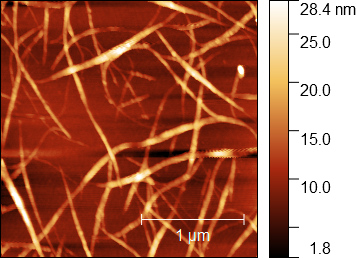
\includegraphics{figures/ch5/Ned_NTQ24_20220125_00235.png}

}

}

\subcaption{\label{fig-bundled-network}Solvent-based deposition}
\end{minipage}%
%
\begin{minipage}[t]{0.05\linewidth}

{\centering 

~

}

\end{minipage}%
%
\begin{minipage}[t]{0.47\linewidth}

{\centering 

\raisebox{-\height}{

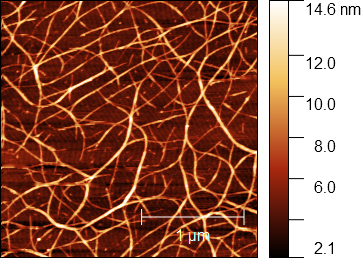
\includegraphics{figures/ch5/Ned_NTQ8C7_w4_pristine_00084_20210428(2).png}

}

}

\subcaption{\label{fig-dropcast-network}Dropcast surfactant-based
deposition}
\end{minipage}%
\newline
\begin{minipage}[t]{0.26\linewidth}

{\centering 

~

}

\end{minipage}%
%
\begin{minipage}[t]{0.47\linewidth}

{\centering 

\raisebox{-\height}{

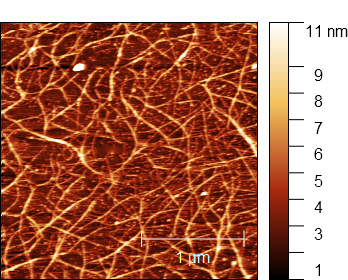
\includegraphics{figures/ch5/Ned_NGQ14D2_W4_pristine_20220713_00567.png}

}

}

\subcaption{\label{fig-steaming-network}Steam-assisted dropcast
surfactant-based deposition}
\end{minipage}%
%
\begin{minipage}[t]{0.26\linewidth}

{\centering 

~

}

\end{minipage}%

\caption{\label{fig-afm-morphology}2.5 \(\mu\)m \(\times\) 2.5 \(\mu\)m
atomic force microscope images of carbon nanotube films deposited using
various methods. NOTE NEED TO ADD EXAMPLES OF SURFACTANT BASED
DEPOSITION POST-ANNEALLING!!!}

\end{figure}

The distribution of the deposited carbon nanotubes was modelled to
quantatively understand the effect of the various methods used on the
resulting network morphology. The diameter range of deposited
single-walled carbon nanotubes can be modelled via a normal or Gaussian
distribution {[}@Thanihaichelvan2018; @Liu2013; @Vobornik2023{]}.
However, when we extract and bin the height profiles from the 2.5
\(\mu\)m \(\times\) 2.5 \(\mu\)m AFM images in
Figure~\ref{fig-afm-morphology}, the histograms do not follow a normal
distribution. The AFM histogram shape results from the SiO\(_2\)
substrate and carbon nanotubes both exhibiting a degree of surface
roughness, which is partially due to the presence of atmospheric
contaminants. In the case of the surfactant-deposited networks, residual
surfactant may also contribute to surface roughness {[}@Vobornik2023{]}.

It has been demonstrated that the surface roughness of a bare SiO\(_2\)
substrate can also be modelled with a normal distribution. This normal
distribution has a spread of approximately \pm1 nm about the mean, which
can be set as the reference or zero point for other height measurements
{[}@Velicky2015{]}. As both the carbon nanotube and silicon dioxide
background heights can each be modelled using a normal distribution, we
therefore assume that a linear combination of normal distributions can
be used to model the AFM histograms in Figure~\ref{fig-afm-morphology}.

\begin{figure}

\begin{minipage}[t]{0.47\linewidth}

{\centering 

\raisebox{-\height}{

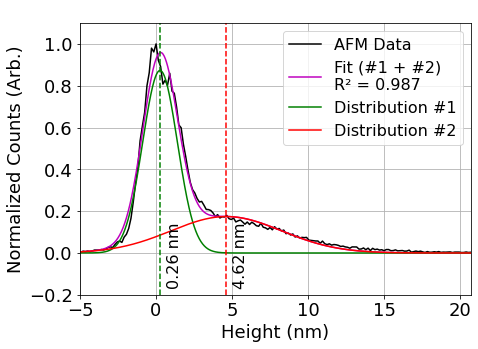
\includegraphics{figures/ch5/Ned_NTQ24_20220125_00235_histogram.png}

}

}

\subcaption{\label{fig-bundled-network-histogram}Solvent based
deposition}
\end{minipage}%
%
\begin{minipage}[t]{0.05\linewidth}

{\centering 

~

}

\end{minipage}%
%
\begin{minipage}[t]{0.47\linewidth}

{\centering 

\raisebox{-\height}{

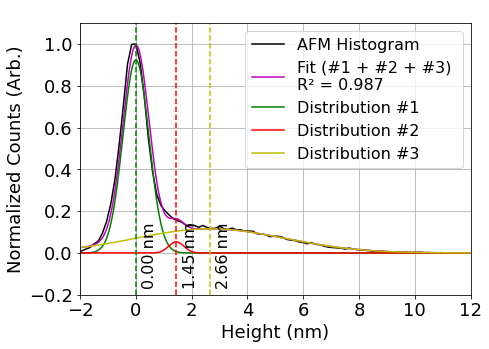
\includegraphics{figures/ch5/Ned_NTQ8C7_w4_pristine_00084_20210428(2)_histogram.png}

}

}

\subcaption{\label{fig-dropcast-network-histogram}Dropcast
surfactant-based deposition}
\end{minipage}%
\newline
\begin{minipage}[t]{0.26\linewidth}

{\centering 

~

}

\end{minipage}%
%
\begin{minipage}[t]{0.47\linewidth}

{\centering 

\raisebox{-\height}{

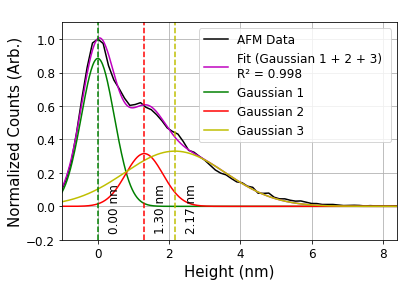
\includegraphics{figures/ch5/Ned_NGQ14D2_W4_pristine_20220713_00567_histogram.png}

}

}

\subcaption{\label{fig-steaming-network-histogram}Steam-assisted
dropcast surfactant-based deposition}
\end{minipage}%
%
\begin{minipage}[t]{0.26\linewidth}

{\centering 

~

}

\end{minipage}%

\caption{\label{fig-afm-histograms}Surface profile histograms extracted
from the 2.5 \(\mu\)m \(\times\) 2.5 \(\mu\)m atomic force microscope
images seen in Figure~\ref{fig-afm-morphology}, each fitted with a
linear combination of normal distributions. The component normal
distributions corresponding to each linear combination are also shown.}

\end{figure}

By using the analysis discussed in \textbf{?@sec-histogram-analysis}, we
find that a linear combination of normal distribution fits to all
histograms corresponding to the AFM images in
Figure~\ref{fig-afm-morphology} with an R-squared value of at least
0.987. The first or left-most distribution for all three figures in
Figure~\ref{fig-afm-histograms} corresponds to the SiO\(_2\) substrate
roughness, centered at \(\sim\) 0 nm and with a standard deviation of
\(0.4-1.2\) nm. For the carbon nanotube film deposited with solvent, the
second distribution then corresponds to bundles of carbon nanotubes. If
we model bundles as cylinders, and we assume the component nanotubes
follow 2D packing and are of equal diameter, we can give an estimate the
mean bundle size in terms of number of nanotubes \emph{n}
{[}@Graham1998; @Thanihaichelvan2018; @Specht2023{]}.

\begin{Shaded}
\begin{Highlighting}[]
\CommentTok{\#|}

\NormalTok{knitr}\SpecialCharTok{::}\NormalTok{opts\_chunk}\SpecialCharTok{$}\FunctionTok{set}\NormalTok{(}\AttributeTok{echo =} \ConstantTok{FALSE}\NormalTok{)}
\FunctionTok{library}\NormalTok{(knitr)}
\FunctionTok{library}\NormalTok{(kableExtra)}

\NormalTok{circle\_packing }\OtherTok{\textless{}{-}} \FunctionTok{read.csv}\NormalTok{(}\StringTok{"tables/ch5/circle\_packing.csv"}\NormalTok{, }\AttributeTok{sep=}\StringTok{","}\NormalTok{)}
\NormalTok{circle\_packing }\OtherTok{\textless{}{-}}\NormalTok{ circle\_packing[}\FunctionTok{rowSums}\NormalTok{(}\FunctionTok{is.na}\NormalTok{(circle\_packing)) }\SpecialCharTok{==} \DecValTok{0}\NormalTok{,]}

\NormalTok{knitr}\SpecialCharTok{::}\FunctionTok{kable}\NormalTok{(circle\_packing, }\AttributeTok{col.names =} \ConstantTok{NULL}\NormalTok{, }\AttributeTok{format =} \StringTok{"simple"}\NormalTok{)}
\end{Highlighting}
\end{Shaded}

\hypertarget{tbl-circle-packing}{}
\begin{longtable}[]{@{}
  >{\raggedright\arraybackslash}p{(\columnwidth - 16\tabcolsep) * \real{0.1053}}
  >{\raggedright\arraybackslash}p{(\columnwidth - 16\tabcolsep) * \real{0.1228}}
  >{\raggedright\arraybackslash}p{(\columnwidth - 16\tabcolsep) * \real{0.0965}}
  >{\raggedright\arraybackslash}p{(\columnwidth - 16\tabcolsep) * \real{0.0965}}
  >{\raggedright\arraybackslash}p{(\columnwidth - 16\tabcolsep) * \real{0.1228}}
  >{\raggedright\arraybackslash}p{(\columnwidth - 16\tabcolsep) * \real{0.1228}}
  >{\raggedright\arraybackslash}p{(\columnwidth - 16\tabcolsep) * \real{0.1228}}
  >{\raggedright\arraybackslash}p{(\columnwidth - 16\tabcolsep) * \real{0.1228}}
  >{\raggedright\arraybackslash}p{(\columnwidth - 16\tabcolsep) * \real{0.0877}}@{}}
\caption{\label{tbl-circle-packing}The first eight optimised ratios of
2D packed circle diameter to encompassing circle diameter, given to 3
s.f. (encompassing circle diameter = \(d\), number of packed circles =
\(n\), approximate packed circle diameter = \(d_n\)).\\
}\tabularnewline
\toprule()
\endhead
\(n\) & \text{2} & \text{3} & \text{4} & \text{5} & \text{6} & \text{7}
& \text{8} & \text{9} \\
\(d\)/\(d_n\) & \text{2.00} & 2.15 & 2.41 & \text{2.70} & \text{3.00} &
\text{3.00} & \text{3.30} & 3.61 \\
\bottomrule()
\end{longtable}

Table~\ref{tbl-circle-packing} shows the relationship between the
diameter of a bundle and the constituent diameters of up to nine 2D
packed carbon nanotubes within that bundle. The second distribution in
Figure~\ref{fig-bundled-network-histogram} indicates the mean diameter
of carbon nanotube bundles is 4.62 nm. Assuming an average carbon
nanotube diameter of 1.45 nm, we find a \(d\)/\(d_n\) packing ratio of
3.19, indicating an average bundle composition of \(\sim\) 7 nanotubes
in Figure~\ref{fig-bundled-network-histogram}.

For the carbon nanotube networks deposited using surfactant in
Figure~\ref{fig-afm-histograms}, we notice that there are two
non-SiO\(_2\) distributions present. The mean of the second
distribution, the left-most non-SiO\(_2\) distribution, falls below the
average height for a single carbon nanotube. This attribute indicates
that the distribution either represents broken pieces of individual
carbon nanotubes, residual surfactant or other atmospheric contamination
resistant to acetone and isopropanol rinsing. This contamination
distribution is significantly larger for the carbon nanotube devices
which used steam in the deposition process. The presence of this
contamination histogram distribution was consistently found for all
sampled surfactant-deposited film AFM data, while not present for any of
the sampled solvent-deposited films.

From Figure~\ref{fig-steaming-network}, we also see that steam deposited
devices have sparsely distributed \(\sim\) 10 nm high features visible
on their surface which are not present for the other films. These
observations may be evidence of trapped water microdroplets on the
surface from the steam, or could be from the steam causing surfactant to
form persistent features on the surface. The size of this central peak
may be useful for determining the extent of contamination in a carbon
nanotube film, discussed further in \textbf{?@sec-contamination}. Such
contamination may or may not have implications for biosensing
suitability, but surfactant contamination could certainly have negative
effects on biological elements sensitive to surfactant.

\hypertarget{tbl-histogram-parameters}{}
\begin{table}
\caption{\label{tbl-histogram-parameters}The mean of histogram distributions across three different samples for
carbon nanotube films deposited using various methods, along with the
mean sample coverage with bundles and mean proportion of multitubed
bundles present. The mean of the carbon nanotube bundle distribution is
shown with an estimate of the number of nanotubes that could pack into
the mean bundle size via 2D packing. }\tabularnewline

\centering
\begin{tabular}{>{\raggedright\arraybackslash}p{2cm}ccccc}
\toprule
\multicolumn{1}{c}{\textbf{ }} & \multicolumn{3}{c}{\textbf{Distribution Mean (nm)}} & \multicolumn{2}{c}{\textbf{Bundle Attributes}} \\
\cmidrule(l{3pt}r{3pt}){2-4} \cmidrule(l{3pt}r{3pt}){5-6}
 & Silicon & Contaminant & Bundles (tubes) & \% multi-tube & \% coverage\\
\midrule
Solvent deposited & 0.1 ± 2.3 & — & 6.2 ± 3.7 (13) & 78 ± 16 & 35 ± 21\\
 &  &  &  &  \vphantom{1} & \\
Surfactant deposited & 0.0 ± 0.4 & 1.0 ± 0.4 & 2.0 ± 1.8 (1) & 27 ± 25 & 31 ± 9\\
 &  &  &  &  & \\
Surfactant deposited with steam & 0.0 ± 0.5 & 1.3 ± 0.6 & 2.0 ± 1.2 (1) & 17 ± 17 & 50 ± 11\\
\bottomrule
\end{tabular}
\end{table}

The distribution means corresponding to each type of deposition method,
averaged across histogram fits from three 2.5 \(\mu\)m \(\times\) 2.5
\(\mu\)m atomic force microscope images, are given in
Table~\ref{tbl-histogram-parameters}. The carbon nanotube bundle mean is
given alongside the number of carbon nanotubes corresponding to the mean
height according to 2D packing as given in
Table~\ref{tbl-circle-packing} and Thanihaichelvan \emph{et al.}
{[}@Thanihaichelvan2018{]}.

It is noticeable that the location of silicon and contamination
distribution means are highly consistent between films. Also notable is
a the large decrease in bundle size when surfactant is used in the
deposition process. There is also a large standard deviation in mean
bundle size seen for solvent deposited devices, corresponding to a wide
range of bundle sizes present on the atomic force microscope images of
the solvent-deposited films.

It is also important to consider that for all figures in
Figure~\ref{fig-afm-morphology}, larger height measurements in the
carbon nanotube distribution include surface contamination on the carbon
nanotubes as well as bundle-bundle junctions. The distribution may also
encompass broken nanotube pieces and some silicon oxide surface
contamination at the low end of the range. When considering the
proportion of single-tube bundles relative to multi-tube bundles, we
exclude heights from the carbon nanotube normal distribution below 1.2
nm, the minimum height of the supplied carbon nanotubes. We also exclude
heights above double the distribution mean, to ignore bundle-bundle
junctions and surface contamination.

We then compare the proportion of the curve below and above 2.9 nm, the
minimum multi-tube bundle size for 1.45 nm diameter nanotubes. By doing
so, we get a rough estimate of the proportion of single- to multi-tube
bundles present on the surface. We can also compare the total area of
the carbon nanotube distribution to the area of the other distributions
to get an estimate of the surface coverage by bundles. These values,
averaged across the histogram fits from three 2.5 \(\mu\)m \(\times\)
2.5 \(\mu\)m atomic force microscope images, are given in
Table~\ref{tbl-histogram-parameters}. It should also be noted that
nanotubes undergo some compression from the AFM tip, so these values are
possibly underestimates. However, the mean values for
surfactant-deposited films are in line with those previously found for
IsoNanotubes-S deposited on silicon oxide using alternative analysis
methods {[}@Vobornik2023{]}.

In Figure~\ref{fig-afm-morphology} and
Table~\ref{tbl-histogram-parameters}, we see that carbon nanotubes
deposited in a surfactant dispersion form bundles which are
significantly less wide than the bundles in the film deposited using
solvent. However, we also see that despite the presence of surfactant,
not all surfactant-dispersed carbon nanotubes are deposited
individually. Bundling may occur during the process of deposition onto
the substrate, which could disrupt the repulsive forces from the
surfactant coating and allow attractive forces to temporarily dominate.
The

It is possible that the bundling of surfactant-dispersed carbon
nanotubes occurs due to the coffee-ring effect {[}@Deegan1997;
@VanGaalen2021{]}. The coffee-ring effect refers to a build-up of
dispersed solid forming around the edges of a dispersion evaporating on
a surface. This process occurs due to the dispersion edges being fixed
by surface forces, leading to capillary flow outwards to replace liquid
evaporating at the edges, bringing solid material along with it. The
presence of vapour is known to disrupt this effect {[}@Bishop2020{]}.
Table~\ref{tbl-histogram-parameters} demonstrates that on average, the
presence of steam reduces the number of nanotube bundles present and
increases surface coverage, supporting the above hypothesis.

\hypertarget{sec-pristine-electrical-characterisation}{%
\subsection{Electrical
Characteristics}\label{sec-pristine-electrical-characterisation}}

\hypertarget{carbon-nanotubes}{%
\subsubsection{Carbon Nanotubes}\label{carbon-nanotubes}}

Each carbon nanotube device fabricated was electrically characterised as
described in \textbf{?@sec-electrical-characterisation}. Figure
Figure~\ref{fig-pristine-cnt-characteristics} displays multi-channel
measurements of representative devices fabricated as described in
\textbf{?@sec-fabrication}. To ensure a consistent comparison, each
device here was encapsulated with AZ\(^\circledR\) 1518 encapsulation
before measurements were taken. The channels which did not exhibit
reliable transistor characteristics are not shown. These non-working
channels were either short, due to metal remaining on the channel after
lift-off, or were very low current, due to a very sparse carbon nanotube
network. Devices shown here with a solvent-deposited carbon nanotube
network were fabricated prior to Jan 2022; devices with a
surfactant-deposited network without steam present were fabricated prior
to Jun 2021; devices with a surfactant-deposited network without steam
were fabricated prior to Sep 2022.

Consistent subthreshold regime behaviour between channels is desirable
for reliable multiplexed biosensing.

\begin{figure}

\begin{minipage}[t]{0.49\linewidth}

{\centering 

\raisebox{-\height}{

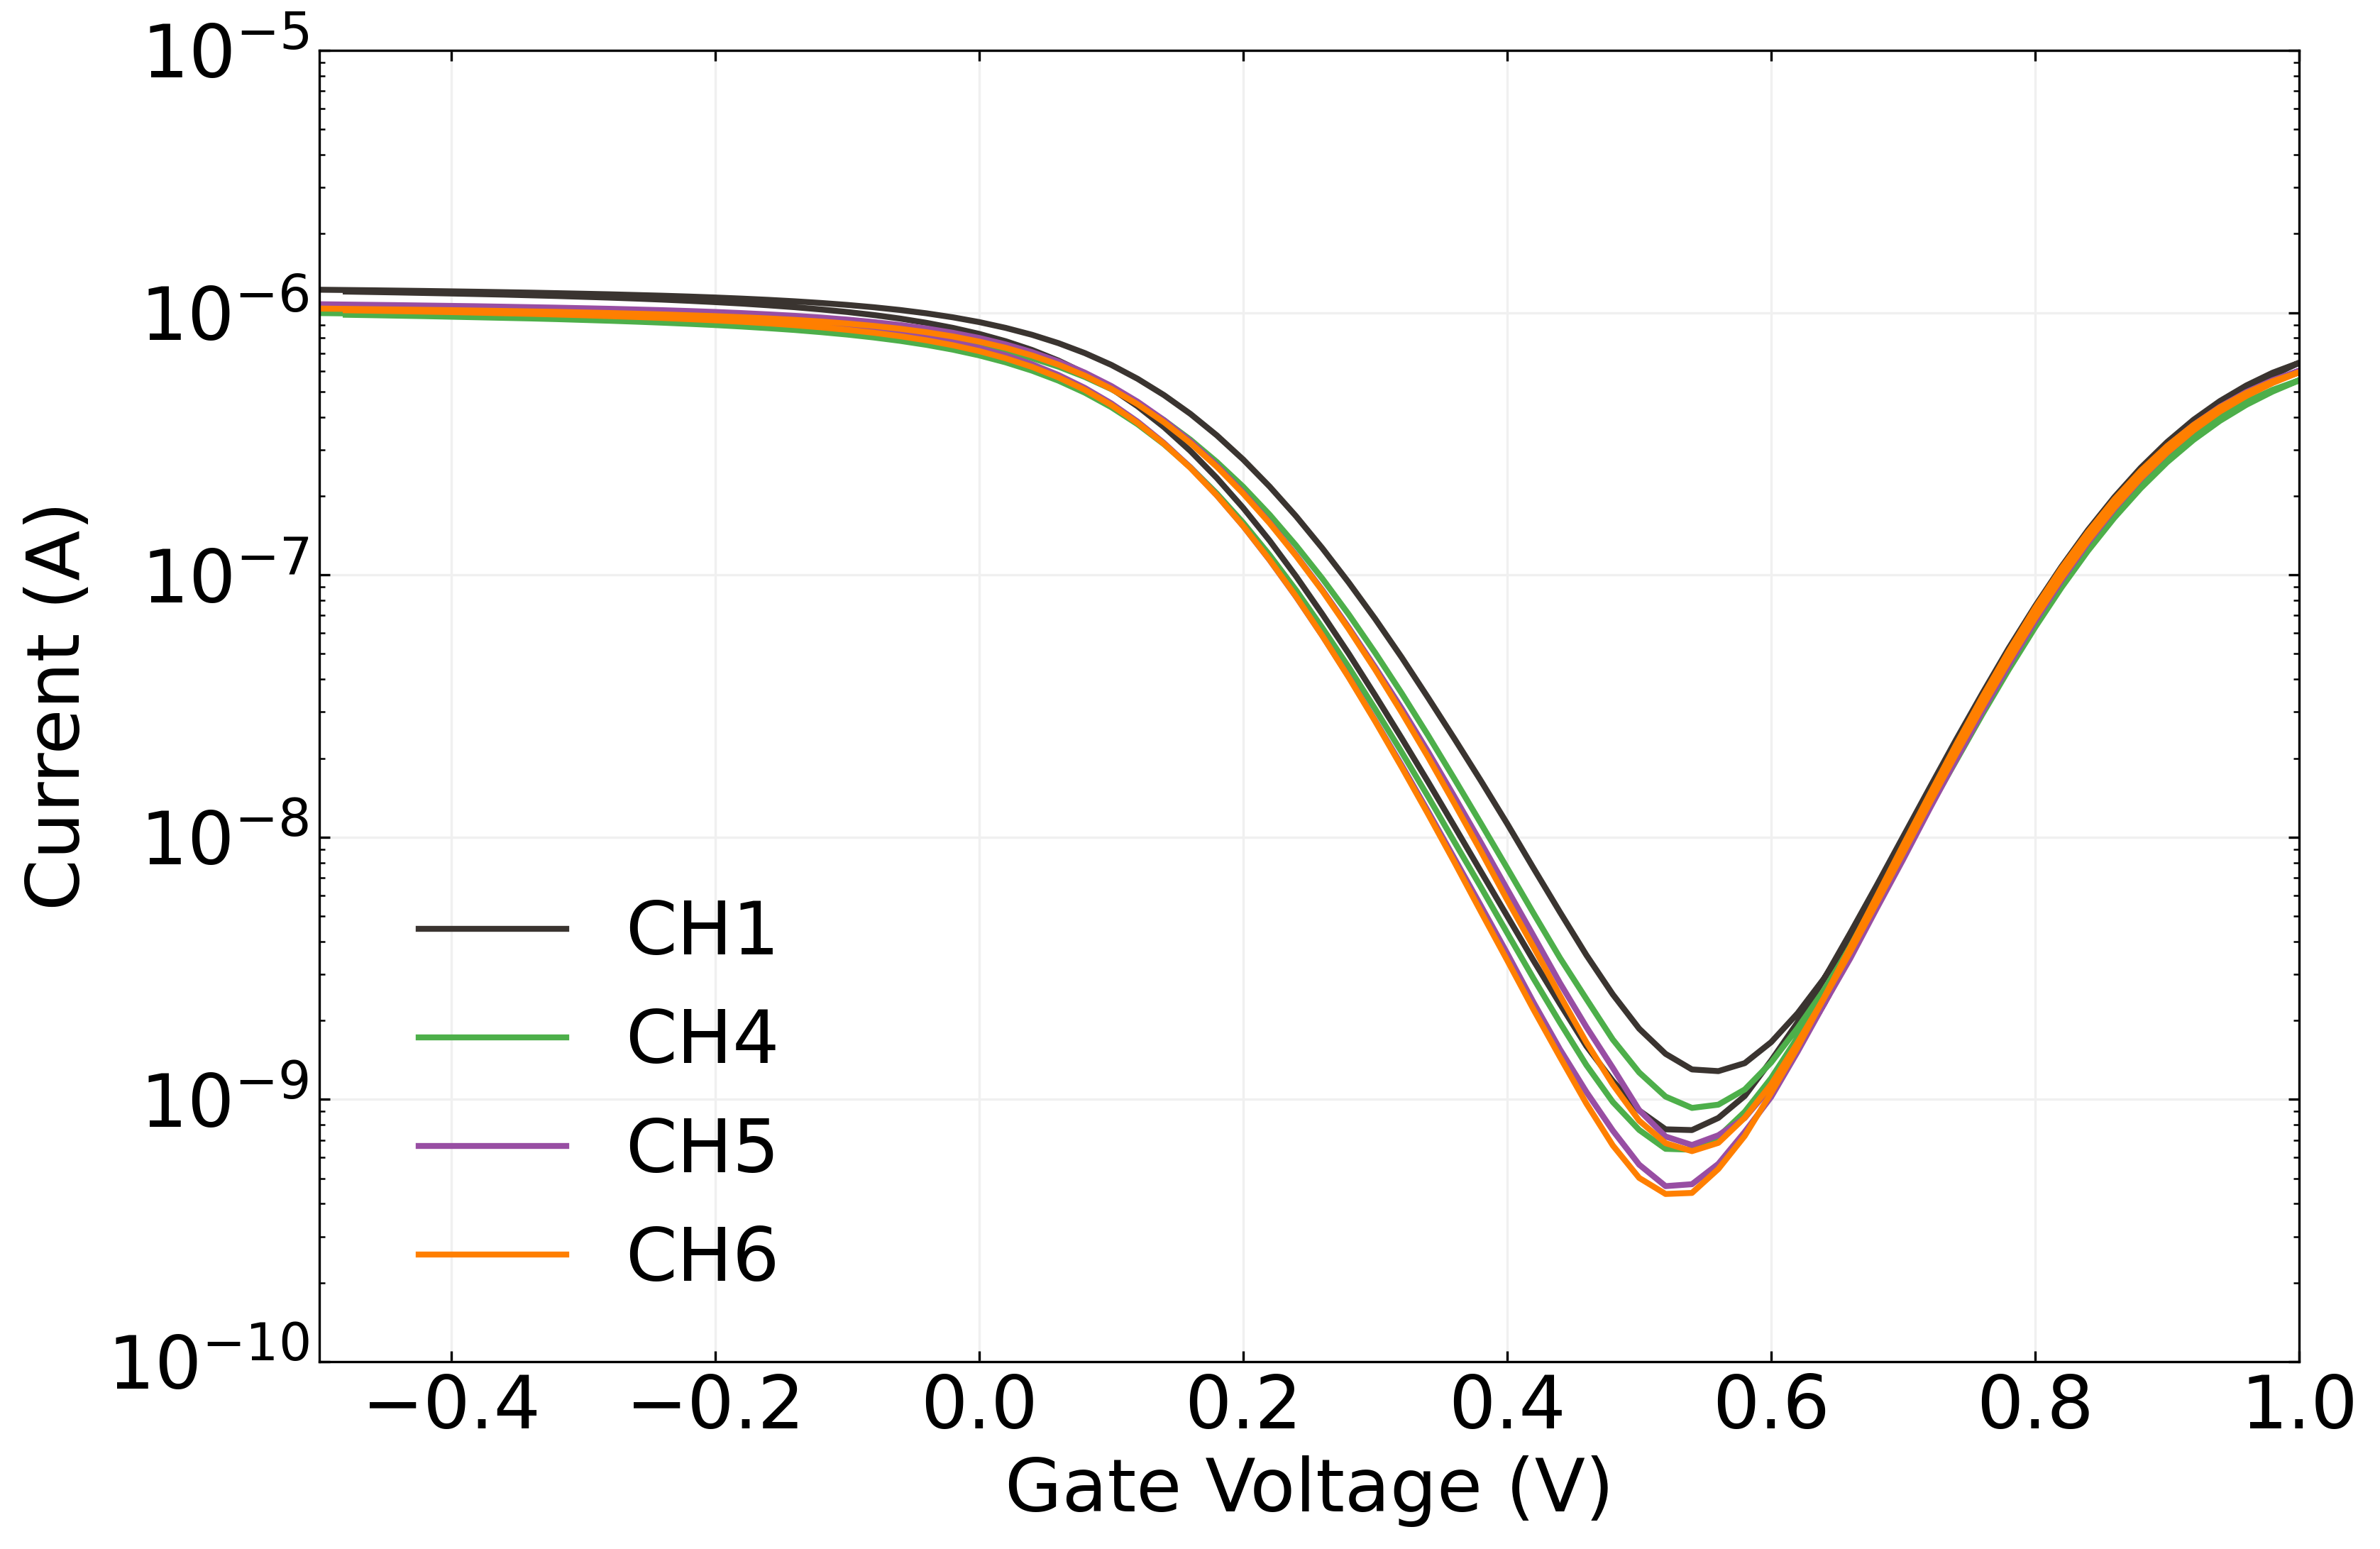
\includegraphics{figures/ch5/NTQ25C7_pristine_TXLG02_220125_solvent_nogate.png}

}

}

\subcaption{\label{fig-solvent-tx-bg}Solvent-based deposition,
back-gated}
\end{minipage}%
%
\begin{minipage}[t]{0.02\linewidth}

{\centering 

~

}

\end{minipage}%
%
\begin{minipage}[t]{0.49\linewidth}

{\centering 

\raisebox{-\height}{

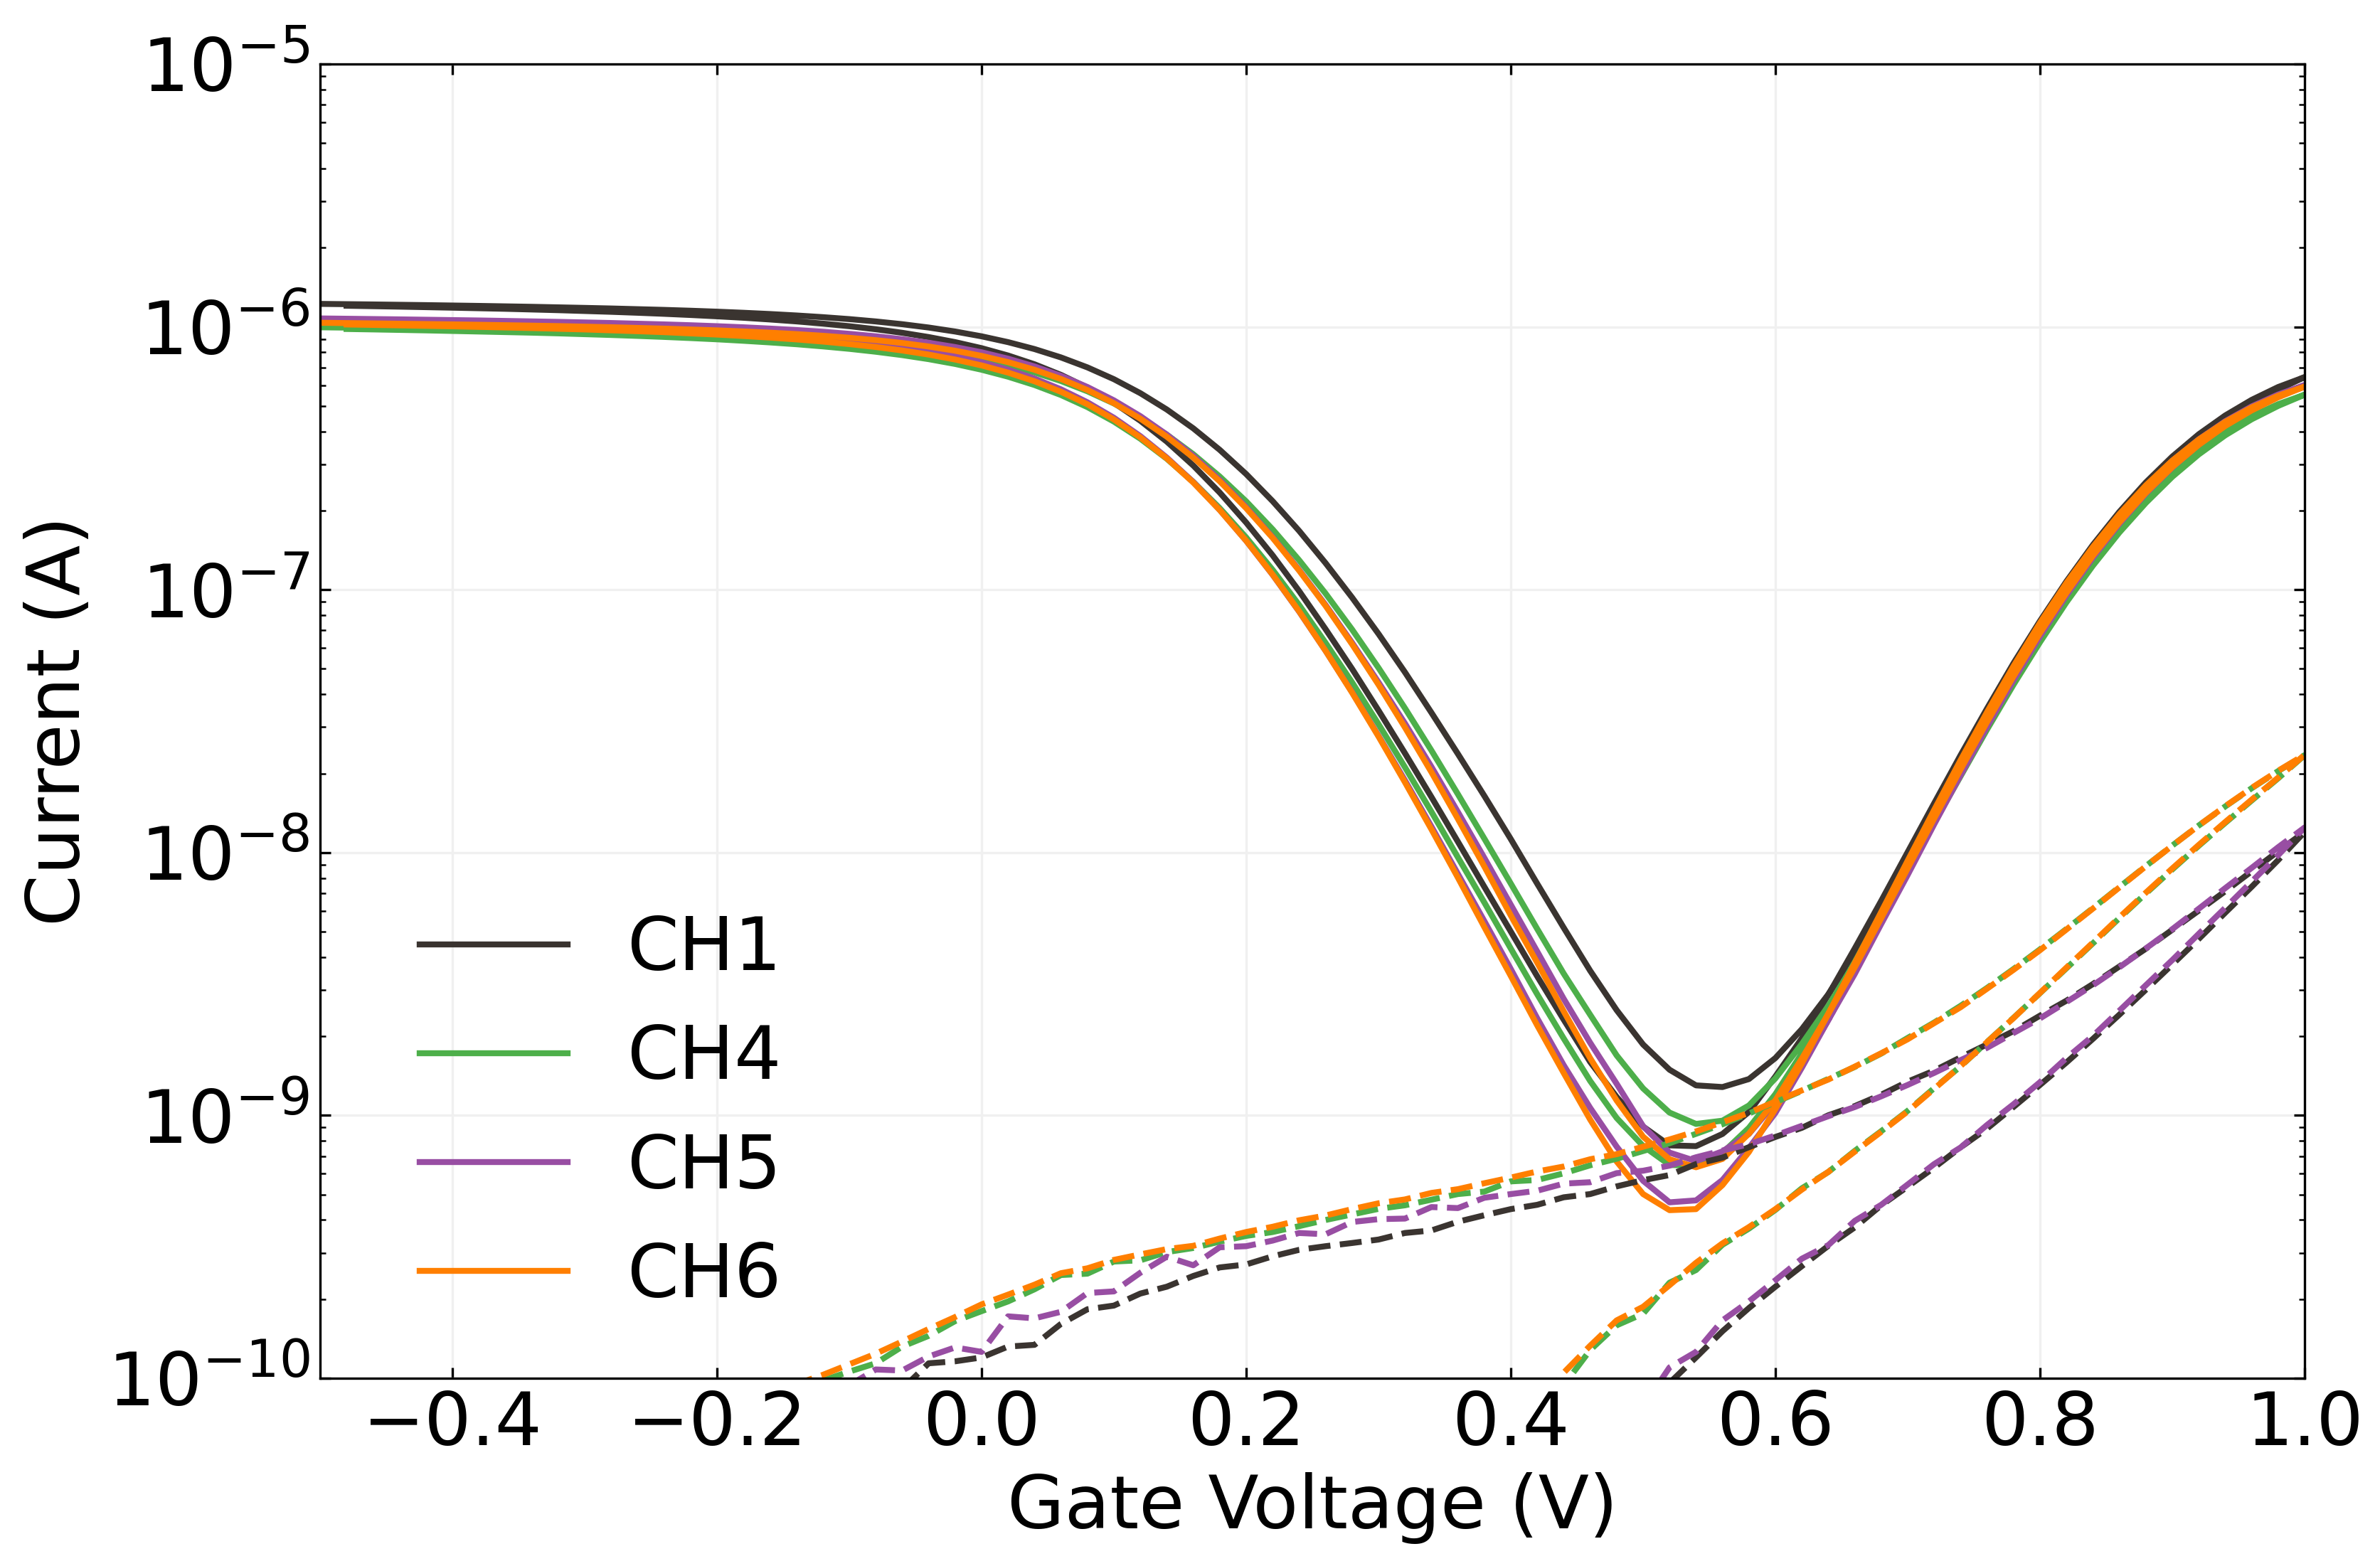
\includegraphics{figures/ch5/NTQ25C7_pristine_TXLG02_220125_solvent_gate.png}

}

}

\subcaption{\label{fig-solvent-tx-tx-lg}Solvent-based deposition,
aqueous-gated}
\end{minipage}%
\newline
\begin{minipage}[t]{0.49\linewidth}

{\centering 

\raisebox{-\height}{

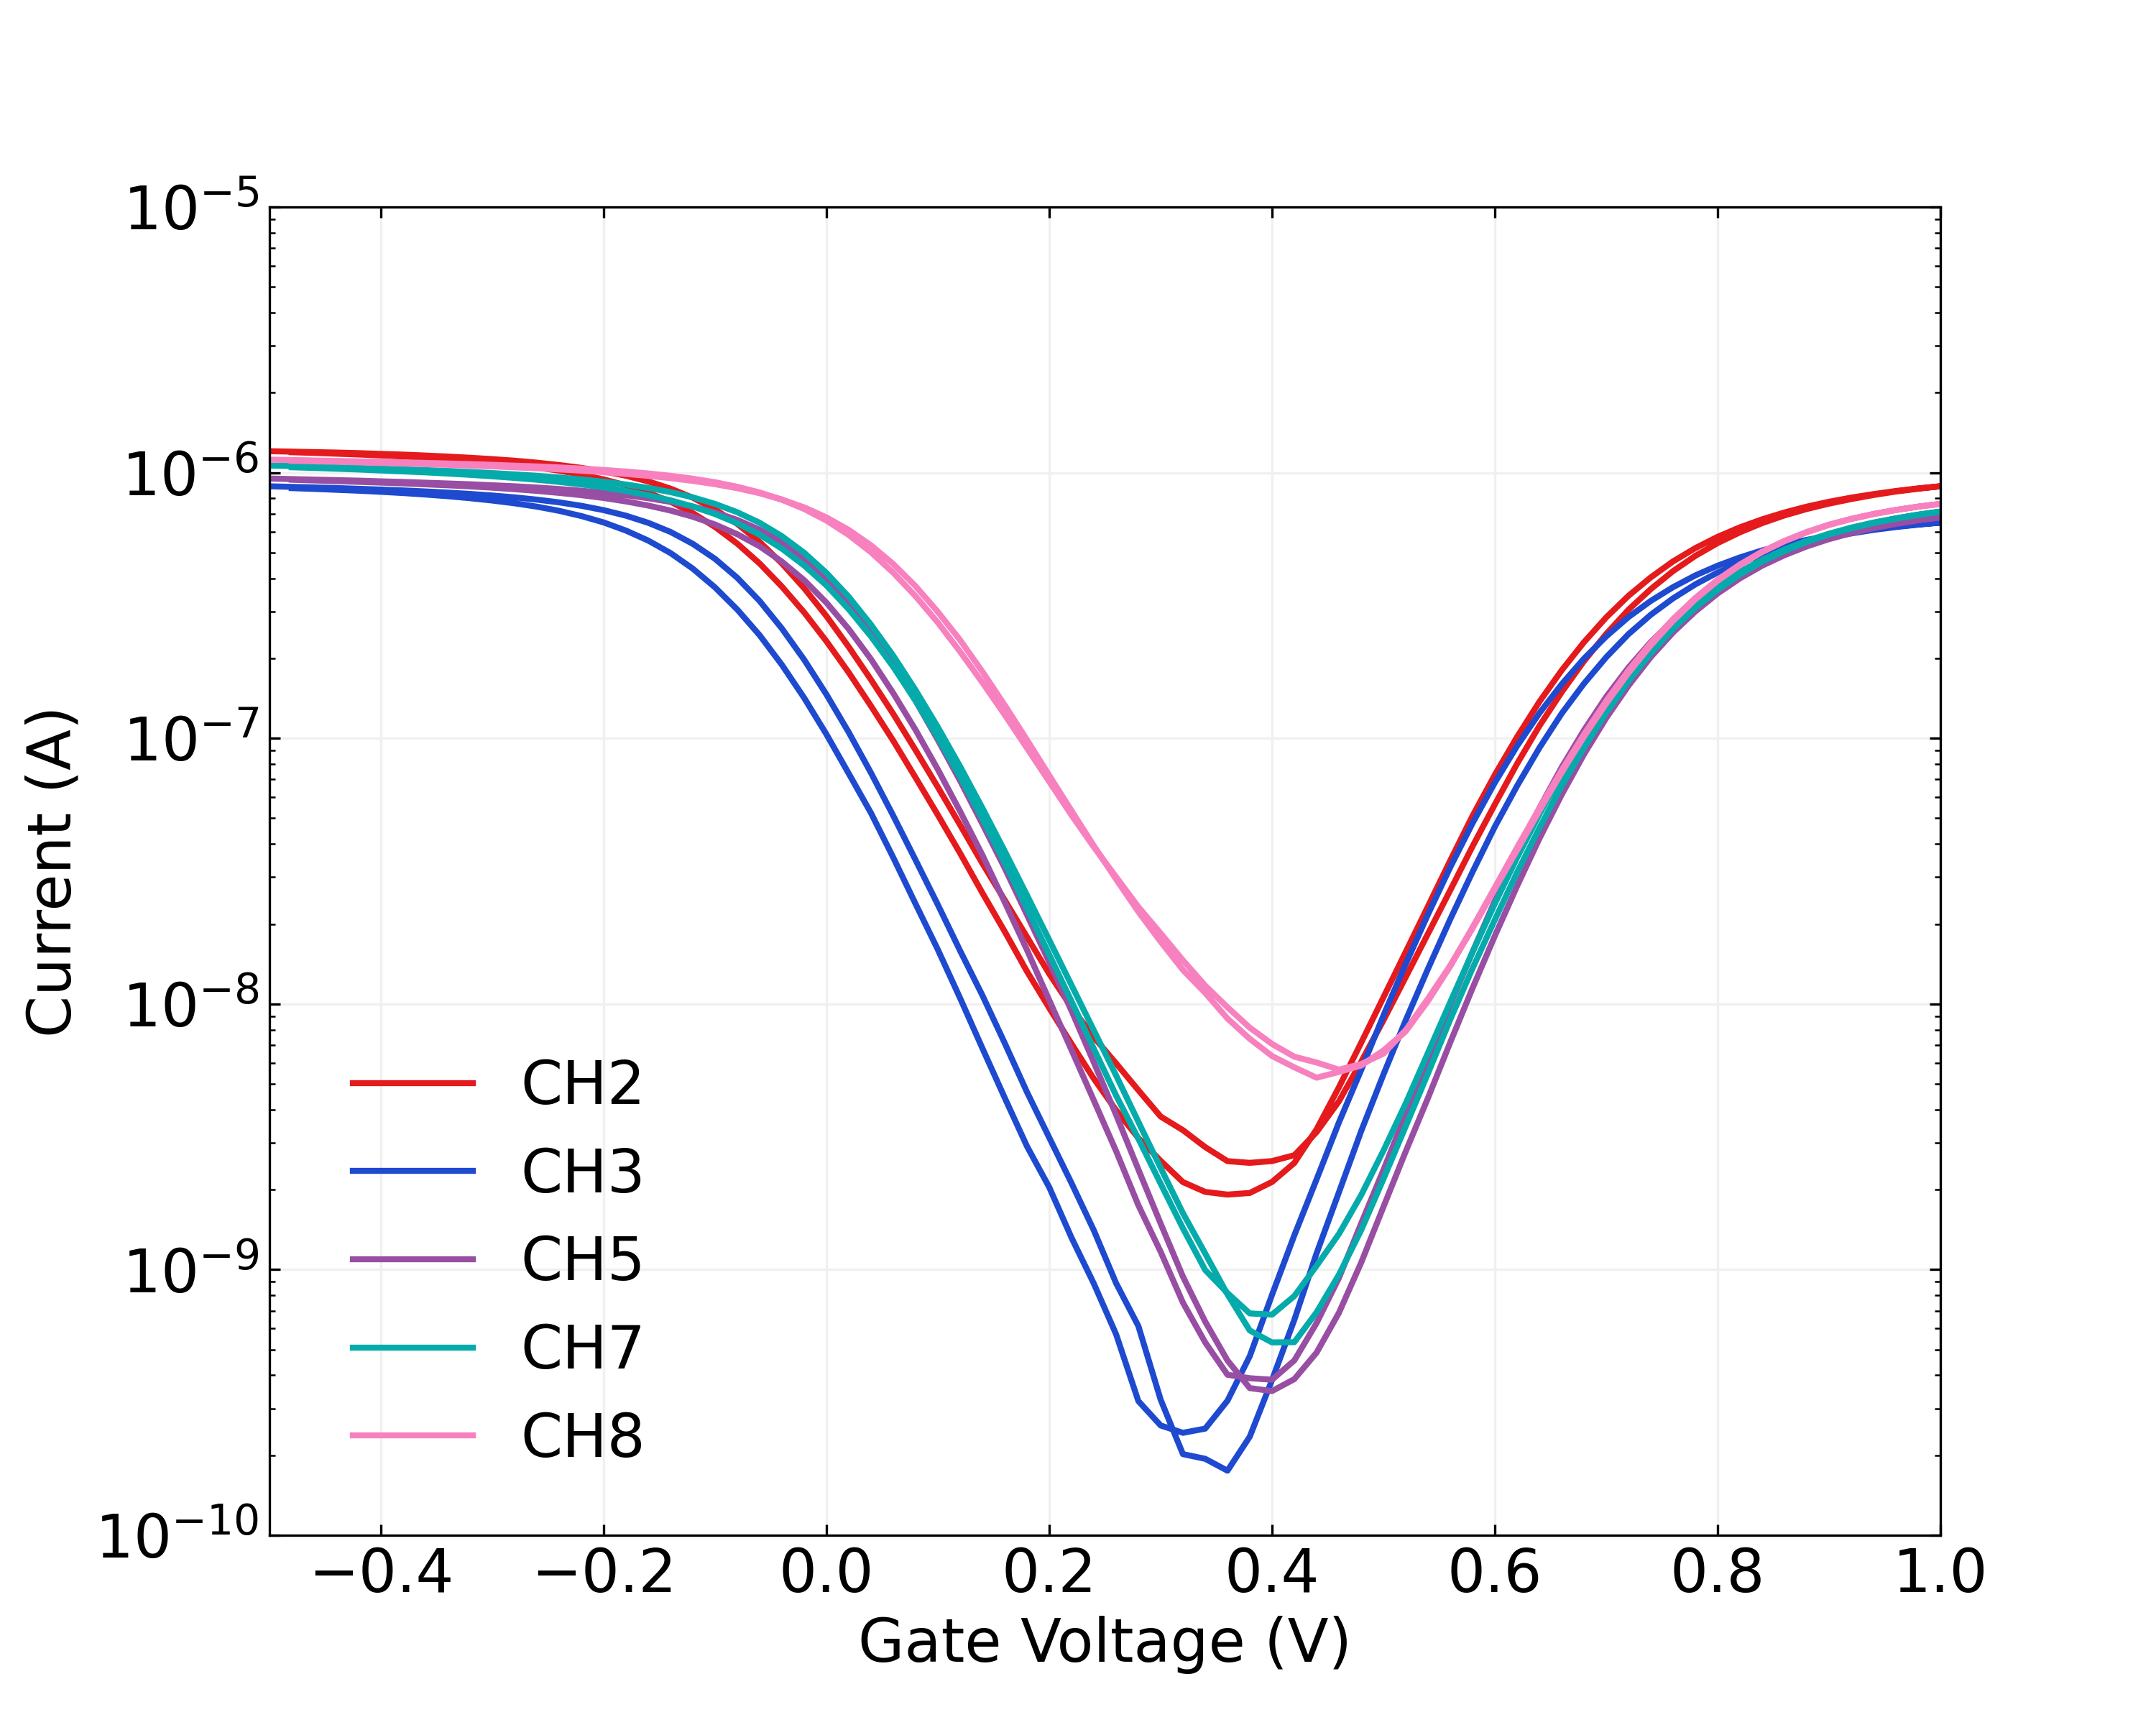
\includegraphics{figures/ch5/NTQ5C3_pristine_TXLG01_210602_nosteam_nogate.png}

}

}

\subcaption{\label{fig-surf-tx-bg}Dropcast surfactant-based deposition,
back-gated}
\end{minipage}%
%
\begin{minipage}[t]{0.02\linewidth}

{\centering 

~

}

\end{minipage}%
%
\begin{minipage}[t]{0.49\linewidth}

{\centering 

\raisebox{-\height}{

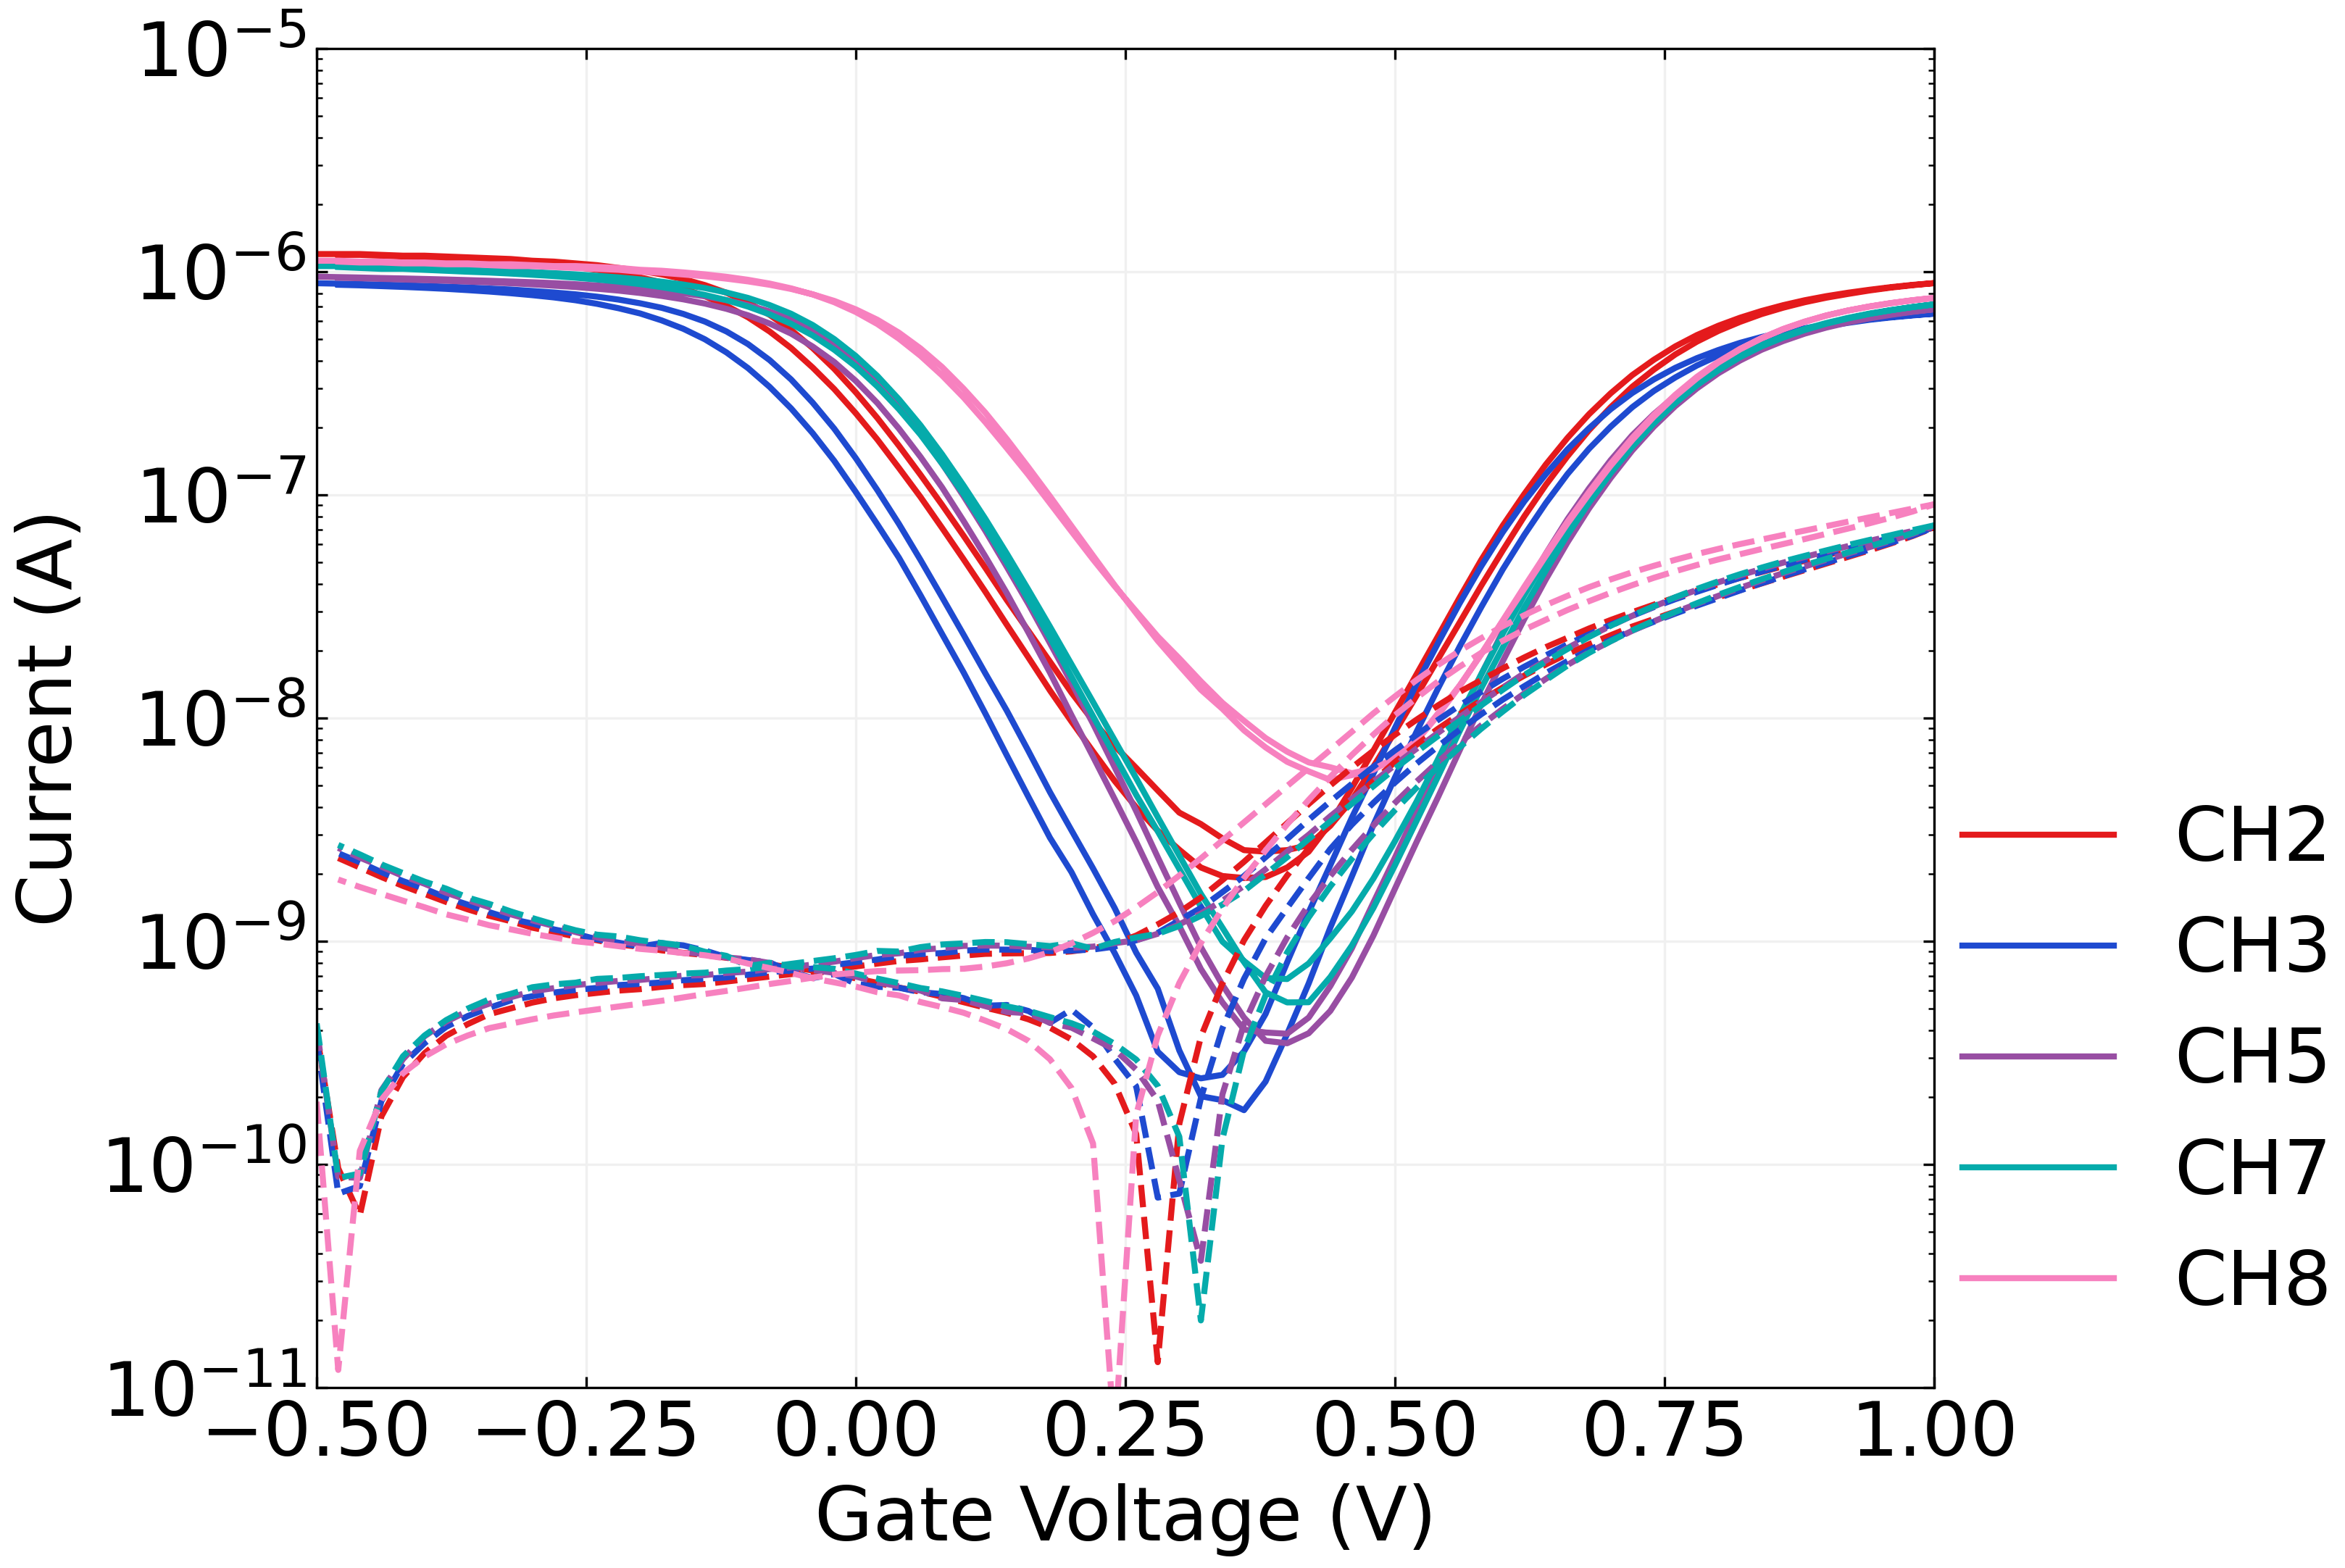
\includegraphics{figures/ch5/NTQ5C3_pristine_TXLG01_210602_nosteam_gate.png}

}

}

\subcaption{\label{fig-surf-tx-lg}Dropcast surfactant-based deposition,
aqueous-gated}
\end{minipage}%
\newline
\begin{minipage}[t]{0.49\linewidth}

{\centering 

\raisebox{-\height}{

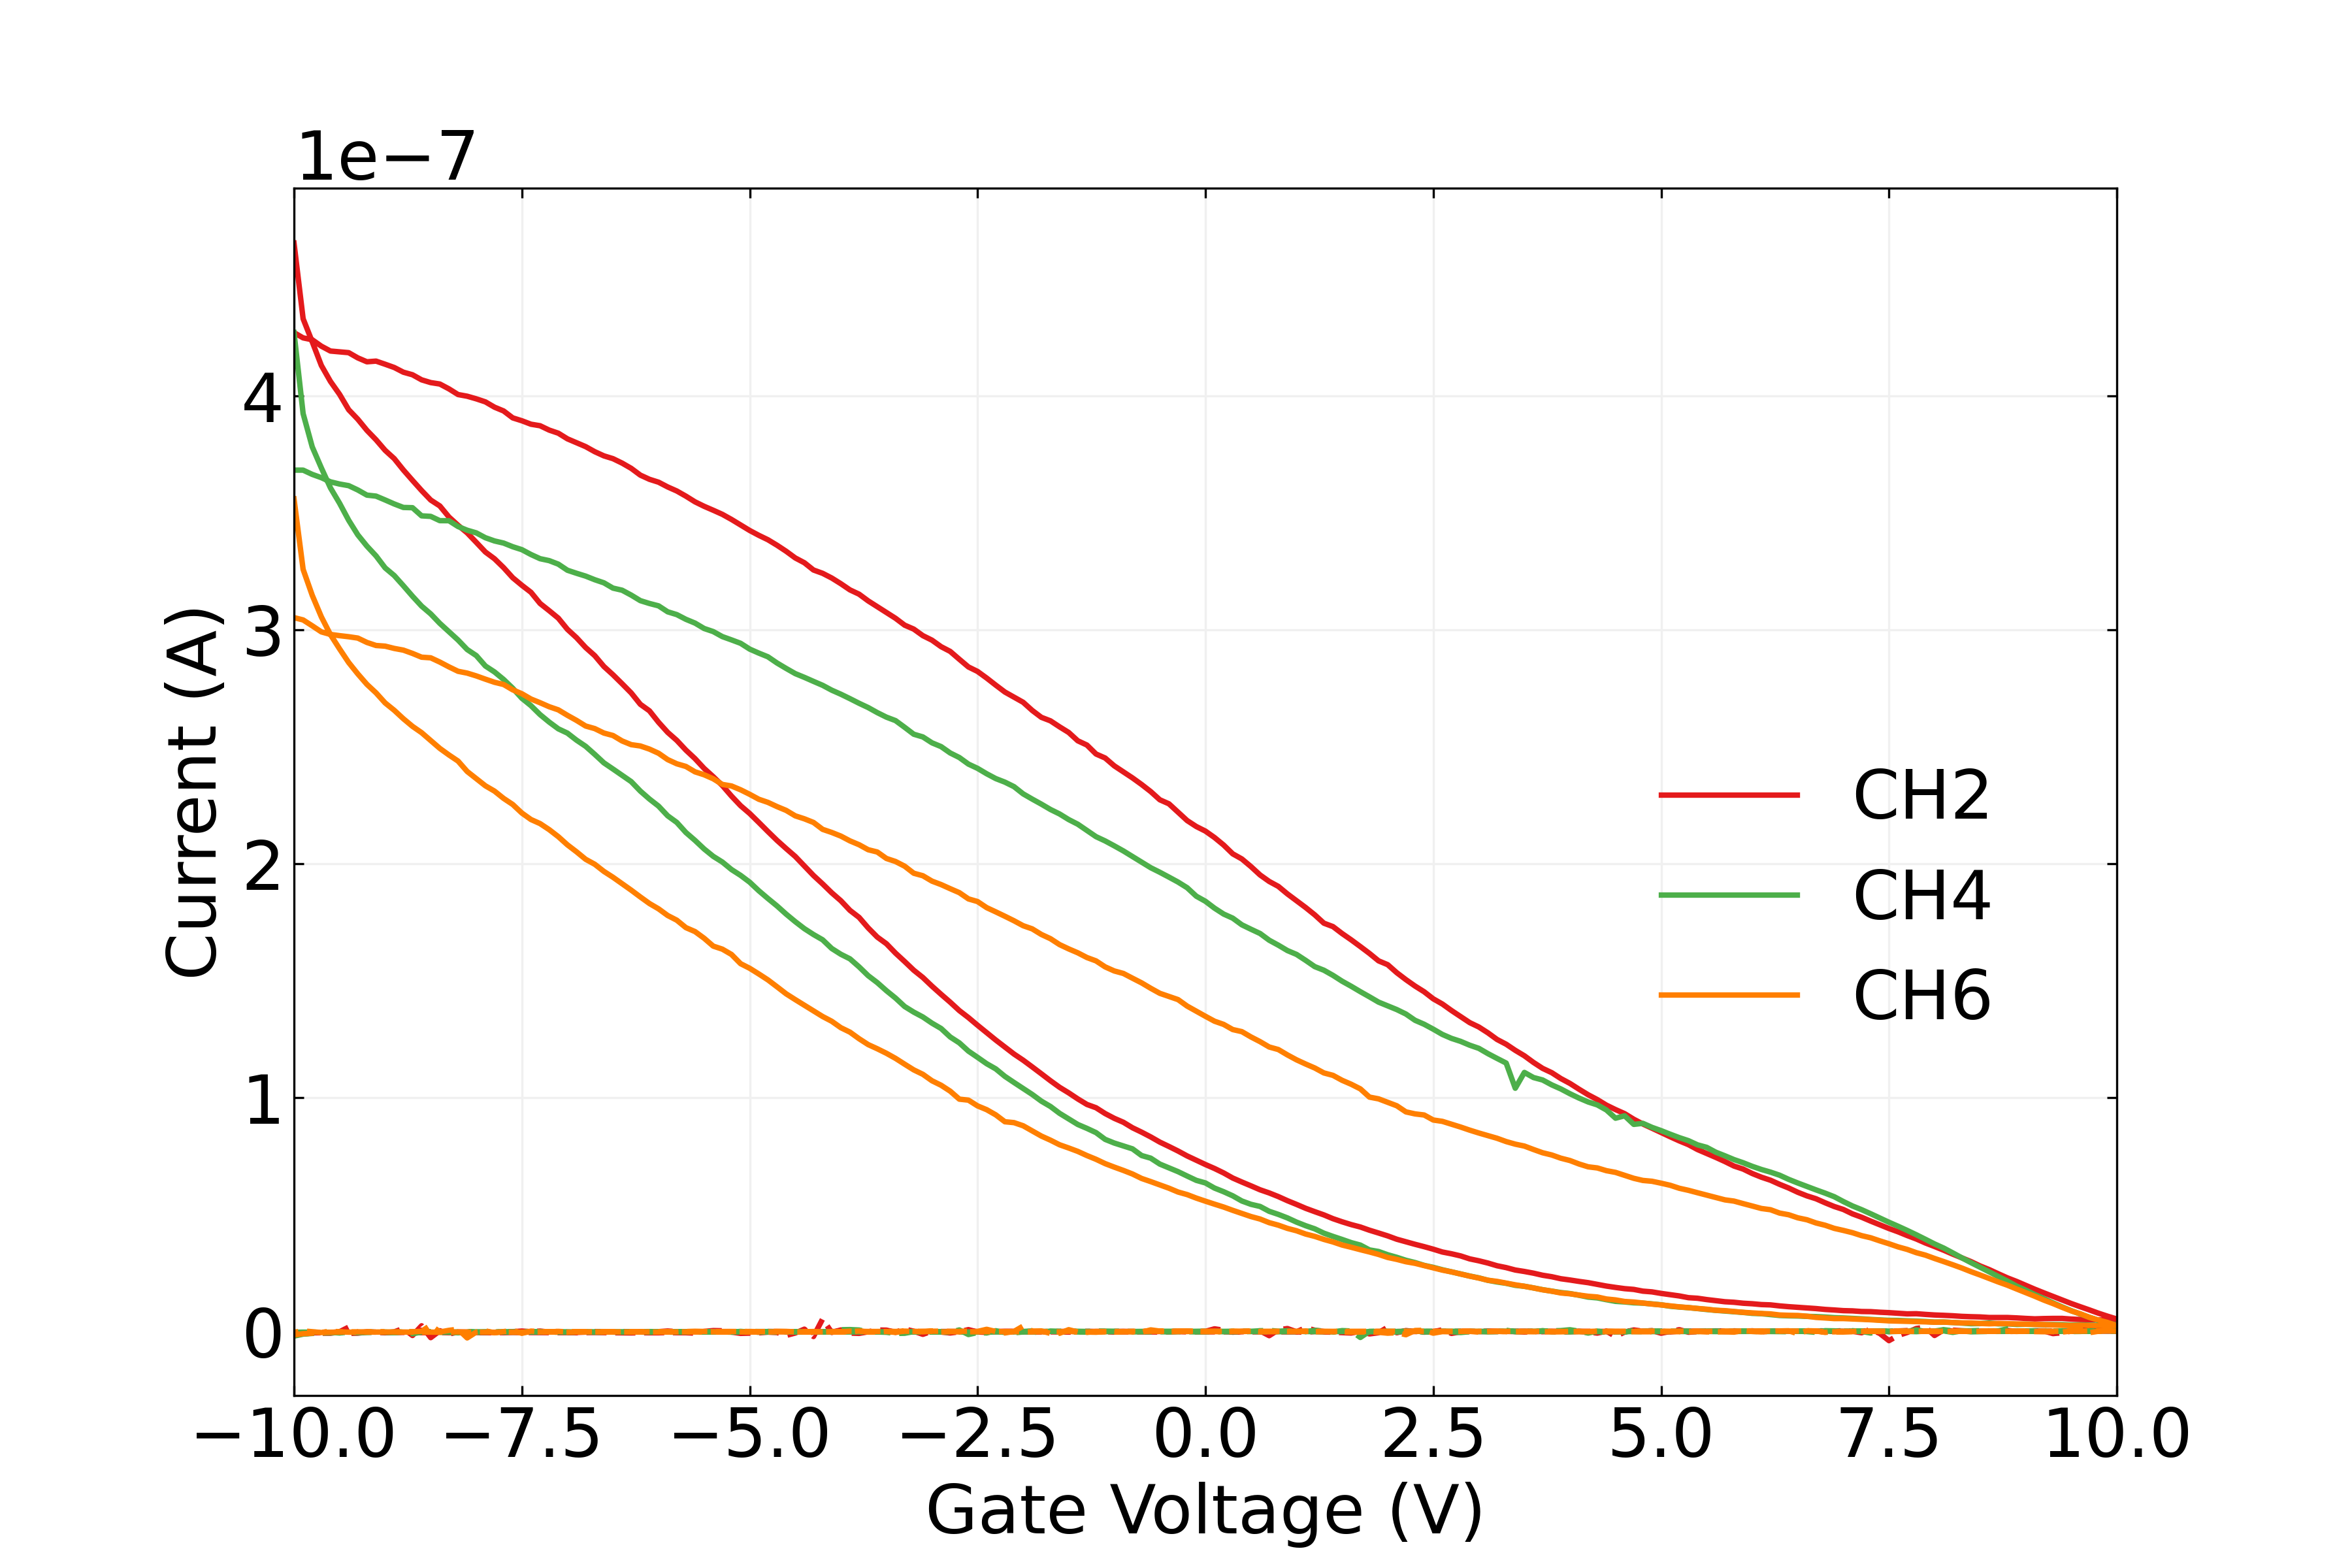
\includegraphics{figures/ch5/Q18C6_steam_backgate.png}

}

}

\subcaption{\label{fig-steam-tx-bg}Steam-assisted dropcast
surfactant-based deposition, back-gated}
\end{minipage}%
%
\begin{minipage}[t]{0.02\linewidth}

{\centering 

~

}

\end{minipage}%
%
\begin{minipage}[t]{0.49\linewidth}

{\centering 

\raisebox{-\height}{

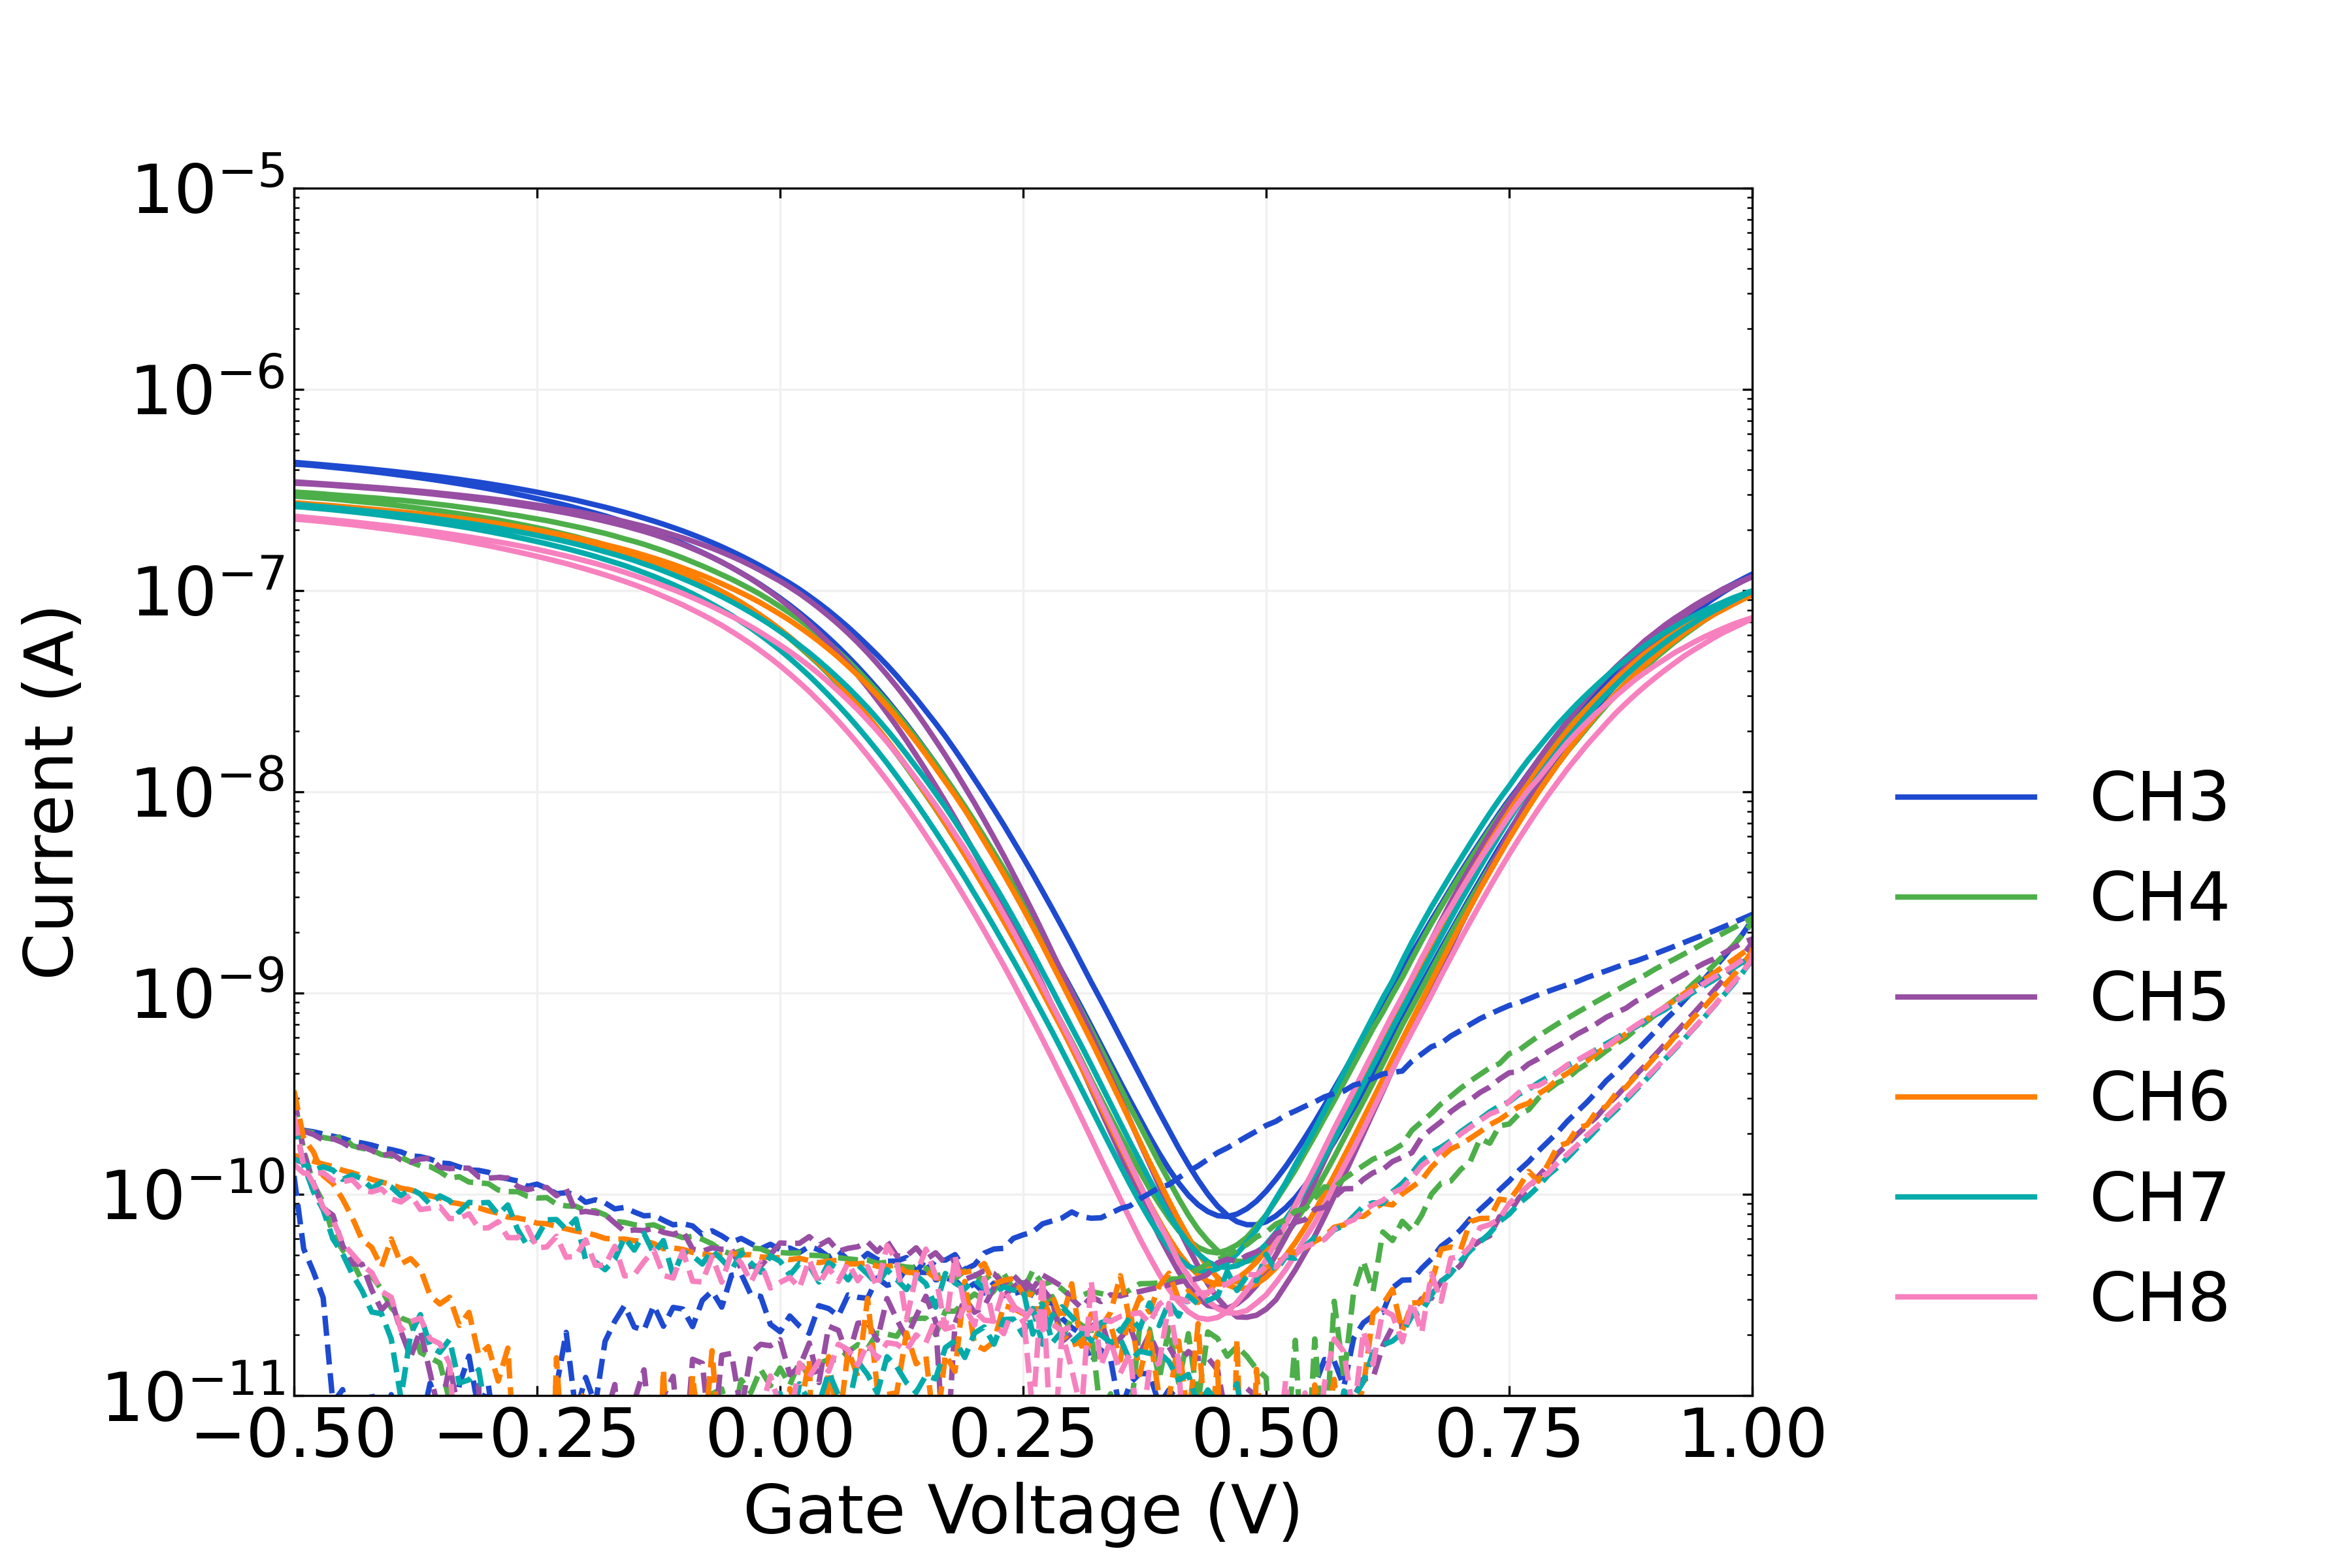
\includegraphics{figures/ch5/NTQ18C1_steam_gate.png}

}

}

\subcaption{\label{fig-steam-tx-lg}Steam-assisted dropcast
surfactant-based deposition, aqueous-gated}
\end{minipage}%

\caption{\label{fig-pristine-cnt-characteristics}Transfer
characteristics of carbon nanotube networks deposited using various
methods. 1XPBS was used as the buffer for the liquid-gated measurements
here. Source-drain voltage used was \(V_{ds} = 100 \textrm{mV}\), with a
step size of either 10 or 20 mV used for the sweep.}

\end{figure}

\hypertarget{sec-dummy-sensing}{%
\subsection{Salt Concentration Sensing with Phosphate Buffered
Saline}\label{sec-dummy-sensing}}

-nLOF2020 resist being used leads to devices with less drift!!



\end{document}
